\begin{figure}[htb!]
\centering
\begin{tabular}{ccc}
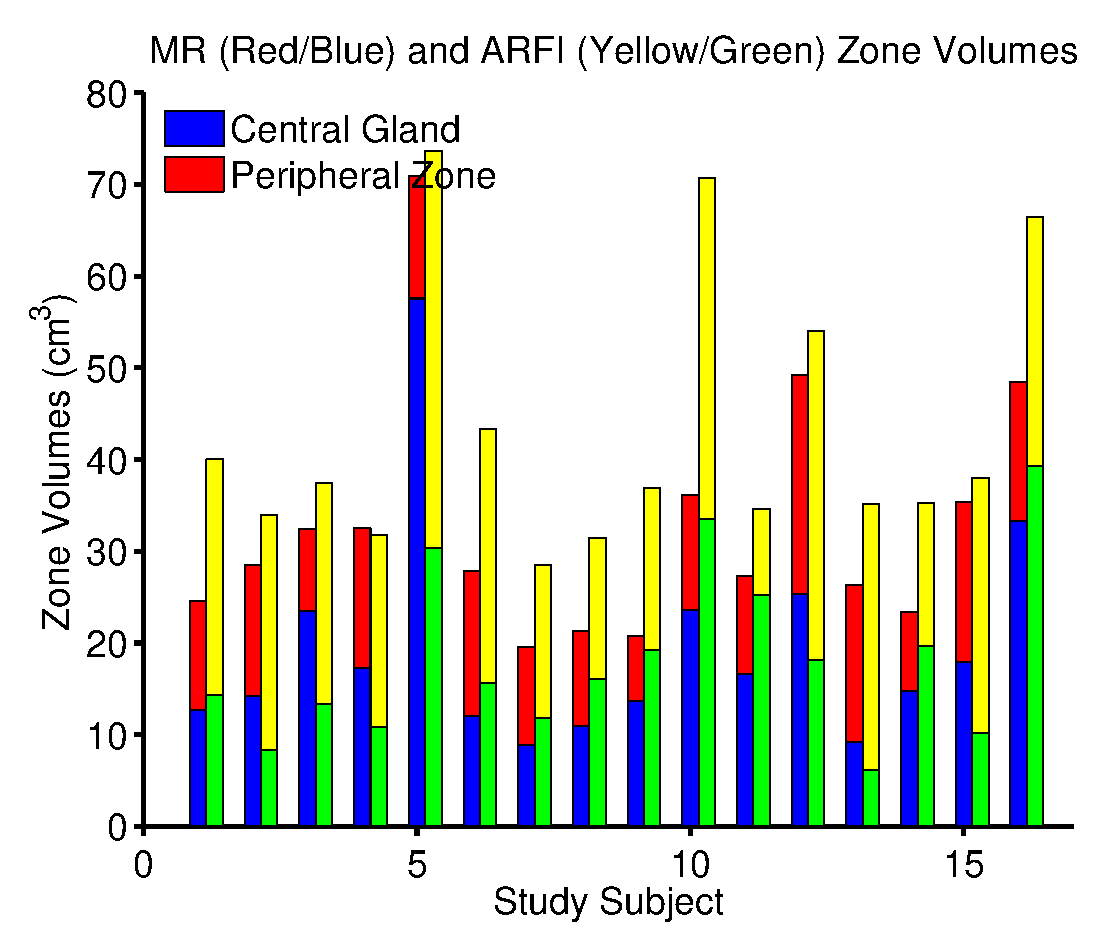
\includegraphics[width=0.3\linewidth]{figs/mr_arfi_volumes} &
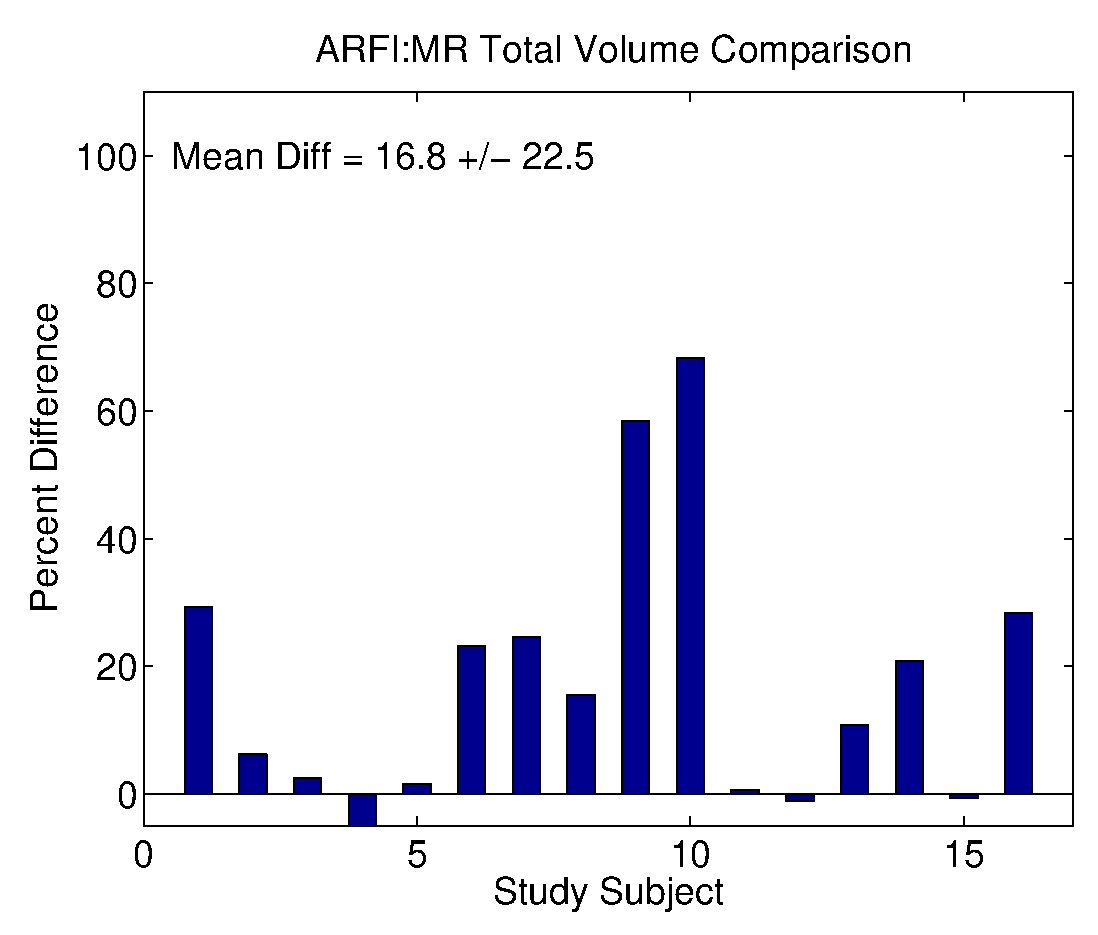
\includegraphics[width=0.3\linewidth]{figs/mr_arfi_volume_diff} &
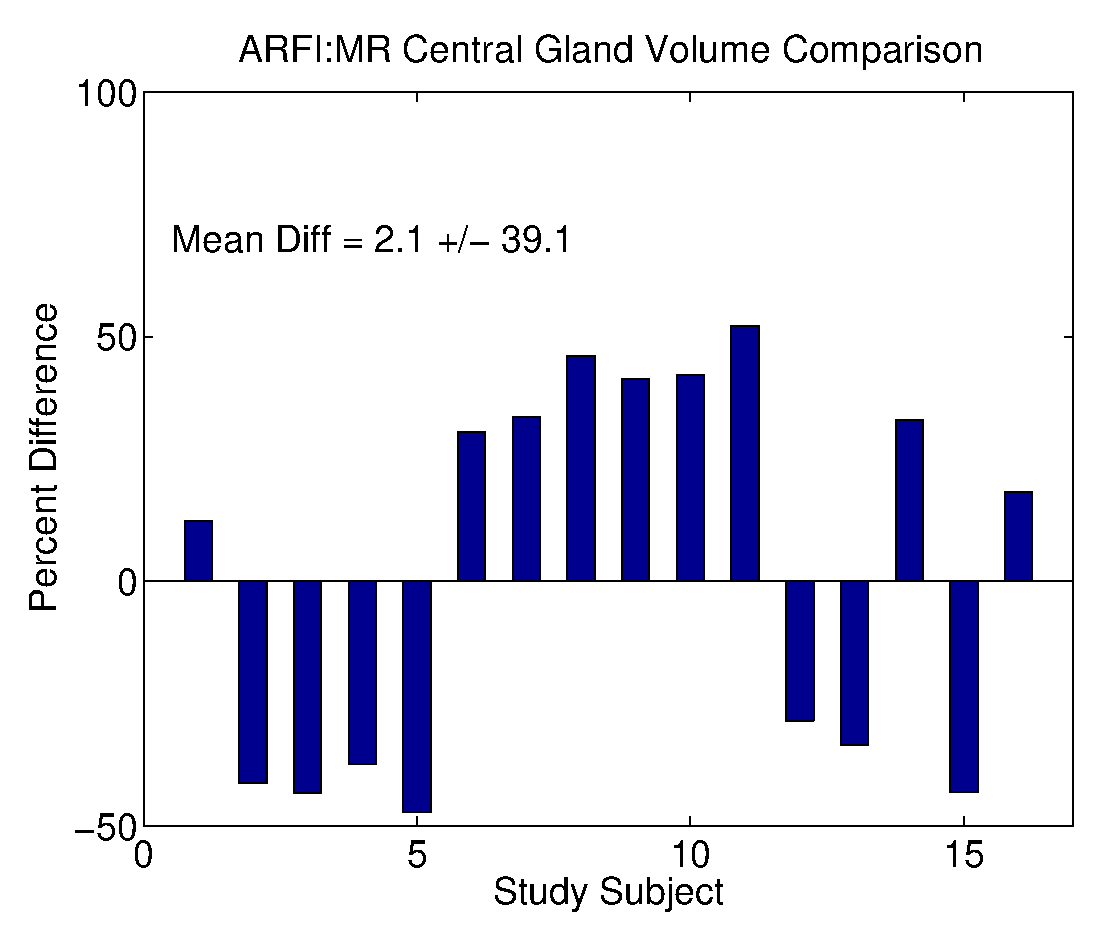
\includegraphics[width=0.3\linewidth]{figs/mr_arfi_central_diff} \\
(a) Central:Peripheral Volume & (b) Total Volume Difference & (c) Central Volume Difference\\
\end{tabular}
\caption{Comparison of MR and ARFI zonal anatomy volume estimates from
    manually-segmented images.  Total prostate volumes ranged from 19.6--71.0
    cm$^3$ based on MR image models (a), with ARFI image models overestimating
    total prostate volume by 36.7 $\pm$ 27.9\% (b).  ARFI image estimation of
    the central zone volume relative to the MR central gland volume varied by
    2.1 $\pm$ 39.0\% (c).  Table~\ref{tab:mr_arfi_volumes} contains the
    individual volume estimates for the entire prostate and the central
    glands.}
\label{fig:mr_arfi_volumes} 
\end{figure}
